\documentclass[a4paper]{article}

%% Language and font encodings
\usepackage[brazilian]{babel}
\usepackage[utf8]{inputenc}
\usepackage[T1]{fontenc}
\usepackage{graphicx}
\graphicspath{{images/}}

%% Sets page size and margins
\usepackage[a4paper,top=3cm,bottom=2cm,left=3cm,right=3cm,marginparwidth=1.75cm]{geometry}

%% Useful packages
\usepackage{amsmath}
\usepackage{graphicx}
\usepackage[colorinlistoftodos]{todonotes}
\usepackage[colorlinks=true, allcolors=blue]{hyperref}

\title{Inferência de distribuição de estratégias no dilema do prisioneiro}
\author{Bruno Vieira Costa}

\begin{document}
	\maketitle

	\begin{abstract}
		Axelrod's tournaments are well-known form of compare Interactive Prisoner's Dilemma strategies in multiplayer scenario. One known result is that the dominant strategy depends on the distribution of strategies participating in the tournament. In this article, I propose a way to infer the distribution of strategies in the game.
	\end{abstract}

	\section{Introdução}
		O dilema do prisioneiro é um dos exemplos clássicos da teoria dos jogos, onde se tem um jogo não coperativo entre duas entidades racionais que pode ser usado para explicar muitos fenômenos complexos na economia.
		Muitas estratégias tem sido desenvolvidas desde a concepção do problema desde heurísticas até técnicas de aprendizado de máquina tem sido empregadas para entender como as diversas estratégias podem interagir com a diversidade mediante a cenários de multiplas interações.
		\\
		Apesar de haver estratégias simples dominantes em muitos cenários, o resultado de torneios é intrinssecamente dependente da distribuição de estratégias dentre os jogadores.
		Neste artigo, será apresentada uma forma de estimar o comportamento aproximado dos jogadores a partir das experiências de um agente autônomo.
		Este método é especialmente útil devido ao conhecimento prévio, mediante a simulações, de estratégias dominantes em diversos contextos.

	\section{Fundamentação teórica}
		\subsection{Dilema do prisioneiro}
			O dilema do prisioneiro é um jogo não coperativo onde duas entidades competem por maximizar suas pontuações mediante a escolhas mais ou menos altruístas.
			Na situação hipotética, dois jogadores escolhem coperar (C) ou delação (D) seu adversário. Neste caso, são possíveis 3 cenários distintos:


			\begin{center}
				\begin{tabular}{| l | l | p{5cm} |}
					\hline
					Jogador 1 & Jogador 2 & Resultado \\ \hline
					C & C & Os dois jogadores ganham uma recompensa (R). \\ \hline
					C & D & O jogador 1 recebe uma recompensa (T) e o jogador 2 recebe uma recompensa (S). \\ \hline
					C & D & O jogador 2 recebe uma recompensa (T) e o jogador 1 recebe uma recompensa (S). \\ \hline
					D & D & Os dois jogadores ganham uma recompensa (P). \\ \hline
				\end{tabular}
			\end{center}

			Em geral, para que haja dilema, é válida a relação

			$$
				T>R>P>S
			$$

			Ou seja, R>P implica que a coperação mútua é mais vantajosa que a delação múltipla. Além disso, T>R e P>S implica que delação seja a estratédia dominante entre os jogadores.

		\subsection{Torneios de Axelrod}
			Em 1980, o cientista político Robert Axelrod convidou alguns teóricos dos jogos para que submetessem suas estratégias em um torneio da versão iterada do dilema do prisioneiro.
			Uma das modalidadesde torneio consiste das seguintes etapas:

			\begin{enumerate}  
				\item São dispostos múltiplos agentes para competir entre si (aos pares).
				\item Retira-se do conjunto os N piores jogadores (soma dos pontos aos pares).
				\item Copia-se os N melhores jogadores.
			\end{enumerate}

			Nesta modalidade de competição, as estratégias puramente agressivas não mais são dominantes por explorarem a vantagem da coperação múltipla.

	\section{Materiais e métodos}
		\subsection{Modelagem}
			Para inferir a estratégia dos oponentes, foi empregada a seguinte aproximação.
			\\
			Cada jogador seguirá a abordagem \textit{Gambler}, onde a decisão será estocástica e dependente somente dos seguintes parâmetros:

			\begin{itemize}  
				\item Primeiros n\textsubscript{1} movimentos do oponente.
				\item Últimos m\textsubscript{1} movimentos do oponente.
				\item Últimos m\textsubscript{2} movimentos do próprios.
			\end{itemize}

			\begin{figure}[h]
				\begin{center}
					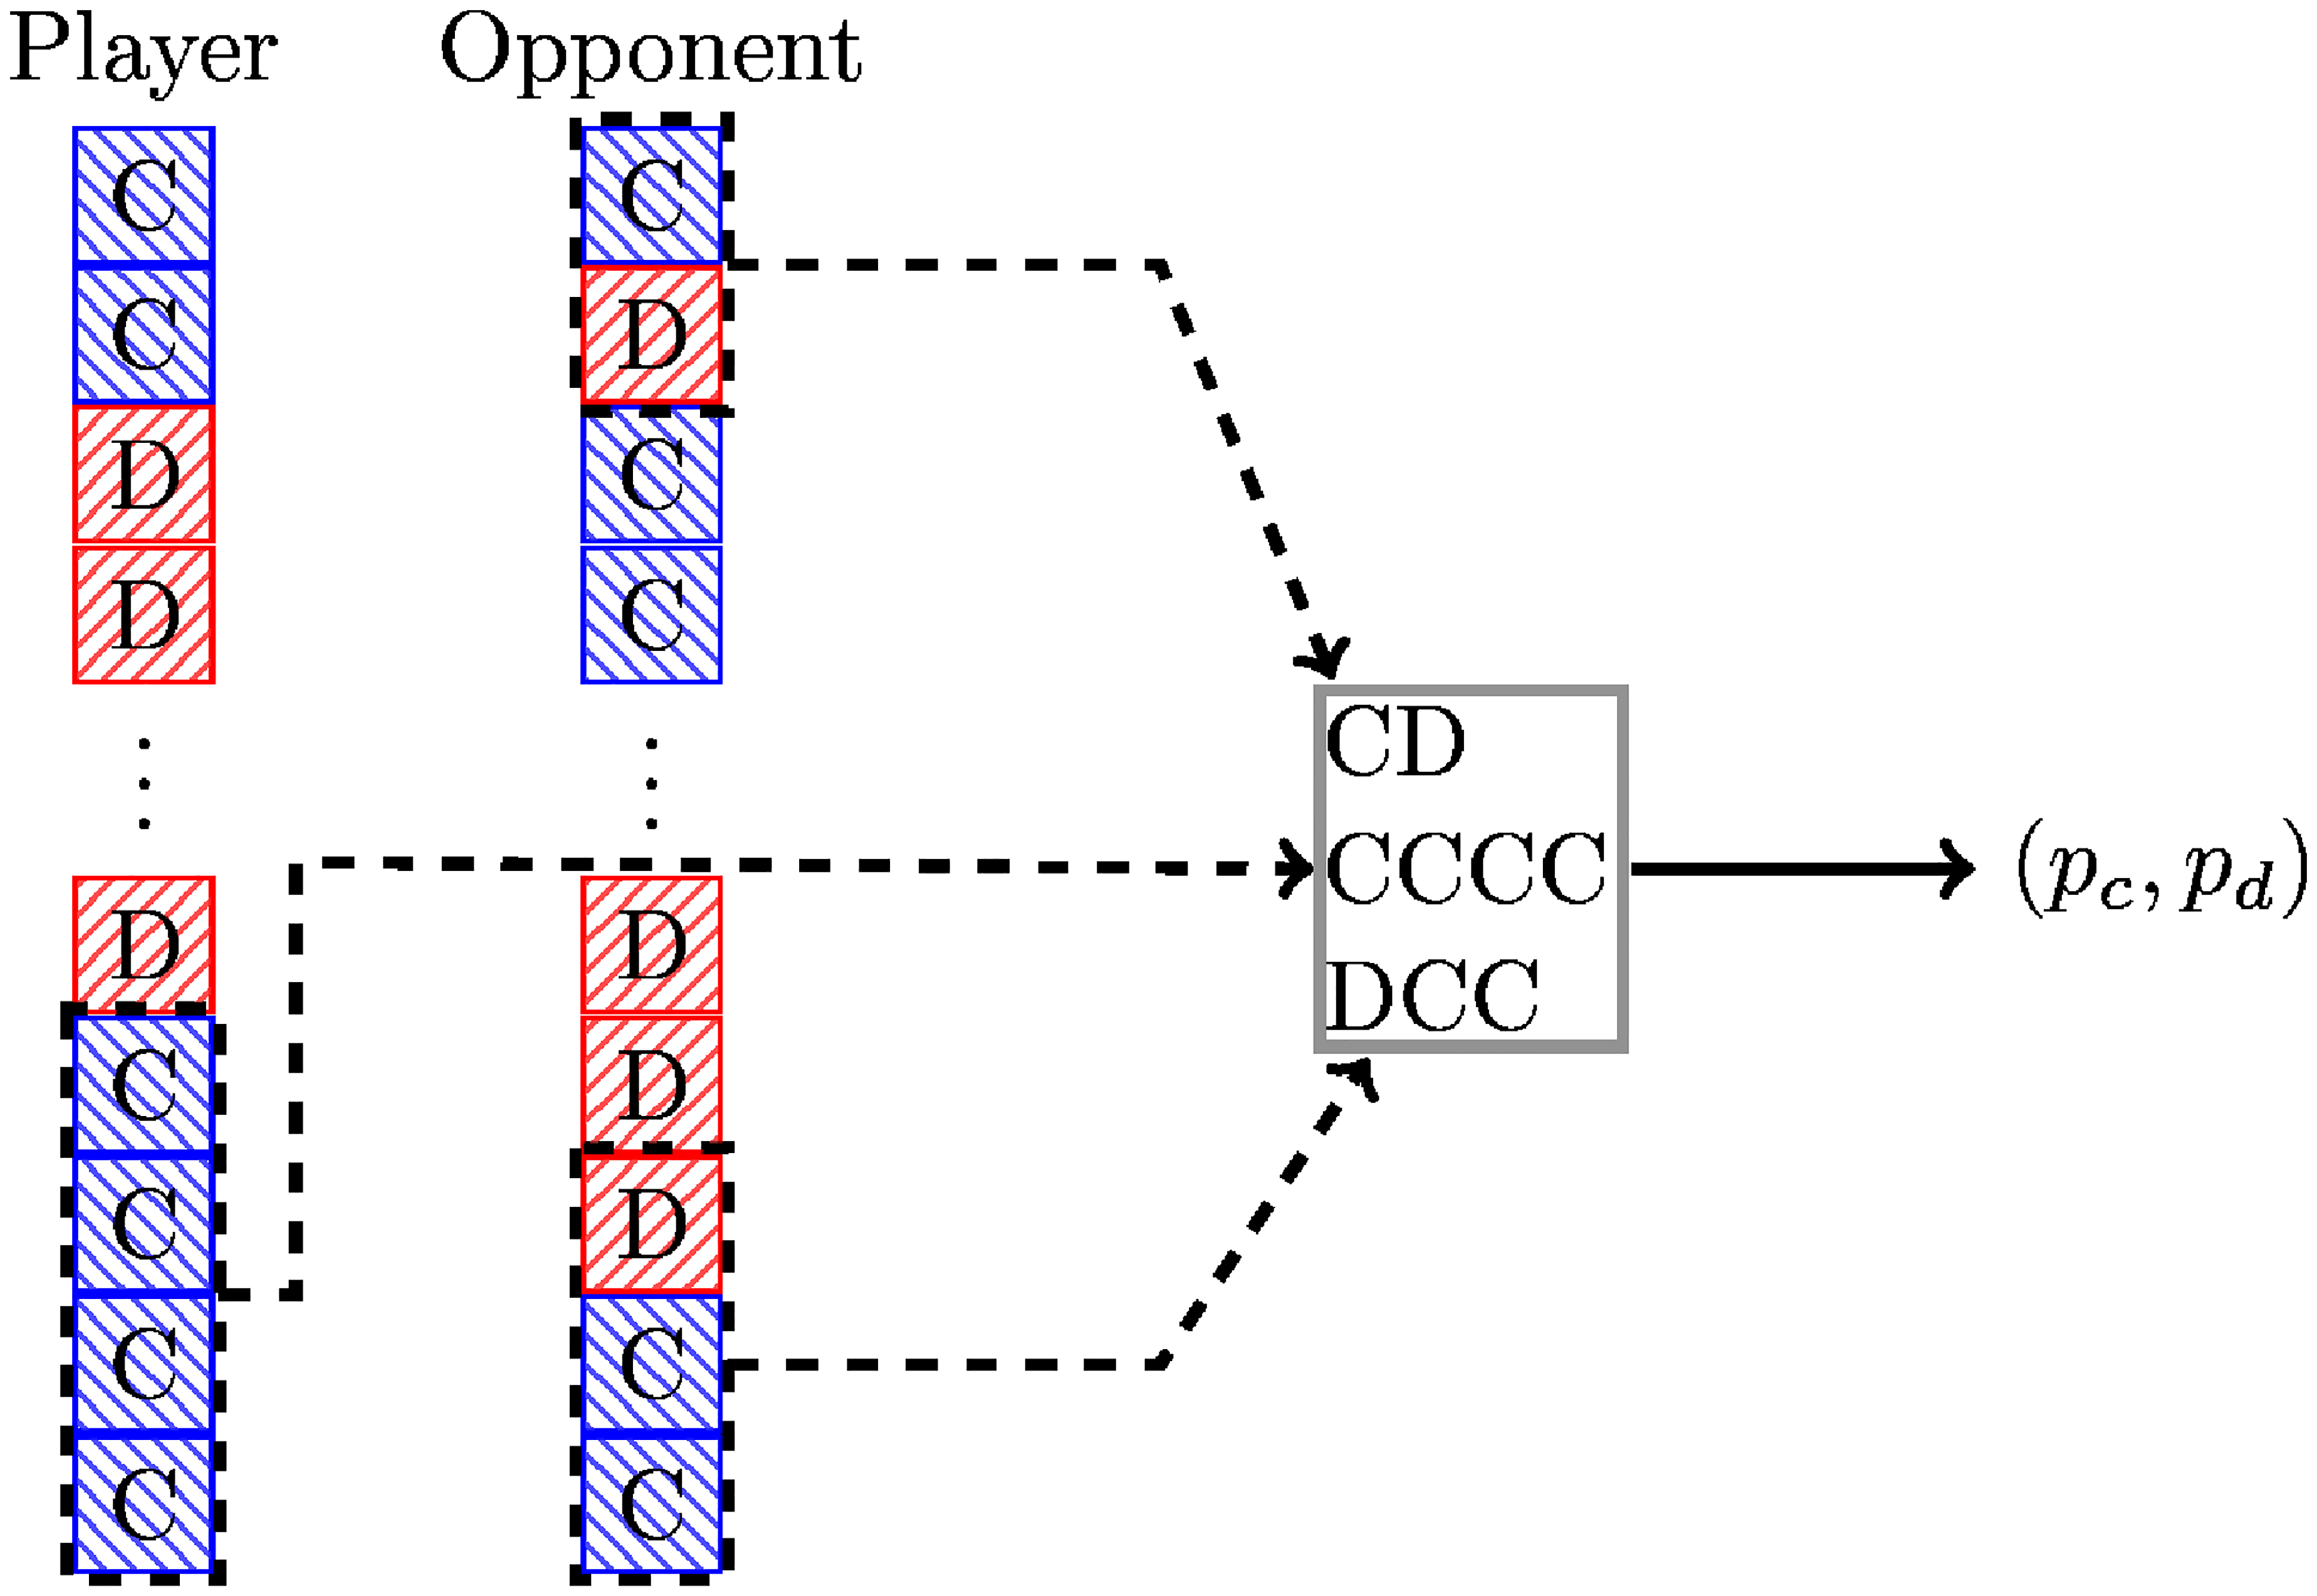
\includegraphics[width=.5\textwidth]{gambler}
				\end{center}
				\caption{Diagrama ilustrativo das estratégias \textit{Gambler}}
			\end{figure}

			Para cada estado de entrada, haverá uma probabilidade de delação ou coperação correspondente.

		\subsection{Aprendizado}
			O algoritmo de aprendizado empregado é feito com umas estrutura de dados de dicionário, onde cada entrada corresponde a uma saida com a quantidade de coperações bem como de delações observadas.
			O agente deverá escolher as primeiras jogadas sempre priorizando preencher as entradas vazias do dicionário.
			\\
			Quando não houver histórico de escolhas suficiente, deve-se utilizar a seguinte aproximação:
			$$
			\begin{cases}
				P(n_1,m_1,m_2) \approx P(max(0,n_1-1),max(0,m_1-1),max(0,m_2-1))
				\\ \\
				P(0,0,0) = \dfrac 1 2
			\end{cases}
			$$

			É estabelecido um limiar de jogadas (M) máximas onde o agente deverá priorizar aprendizado. Após isso, ele deve realizar a ação que otimiza seus ganhos a longo prazo.
		
	\section{Resultados e discussões}
		O algoritmo foi implementado em Python e colocado para teste na framework de Vince Knight que simula as modalidades de torneios de Axelrod.

	\section{Conclusão}
		Nota-se que o algoritmo obtem sucesso em inferir as estratégias mais simples, mas falha ao reconhecer algoritmos mais rebuscados.
		Além disso, o fato de ter muitas jogadas de teste antes da fase de otimização faz com que o algoritmo seja especialmente desfavorável em partidas curtas.

	\begin{thebibliography}{9}
		\bibitem{reinforced} 
			Harper M, Knight V, Jones M, Koutsovoulos G, Glynatsi NE, et al. (2017) Reinforcement learning produces dominant strategies for the Iterated Prisoner’s Dilemma. PLOS ONE 12(12): e0188046. https://doi.org/10.1371/journal.pone.0188046
	\end{thebibliography}

\end{document}
